\documentclass[a4paper,10pt]{article}
\usepackage[utf8]{inputenc}
\usepackage[frenchb]{babel}
\usepackage{graphicx}
\usepackage{amsthm}
\usepackage{amsmath}
\graphicspath{{png/}}
%opening
\title{Algorithmique avancée : Rapport du projet}
\author{FOURNIER Benoit, THIERRY Constance}

\begin{document}

\maketitle

\begin{figure}[b]
\begin{center}

\includegraphics[scale=1]{Enssat.png}
\end{center}
\end{figure}

\thispagestyle{empty}

\newpage
\null
\thispagestyle{empty}
\newpage

\tableofcontents

\hfill

\listoffigures

\newpage
\null
\thispagestyle{empty}
\newpage

\section{Introduction}

La triangularisation de polygone est un problème ()? 
utilisé dans la modélisation 2d et 3d et permet de subdiviser un polygone en un ensemble de triangle.
Nous nous interessons ici au sous-cas des polygone convexe avec pour contrainte une (distance de traingularisation) la plus faible possible.
L'objectif de cette etude est de comparer différentes solutions algorithmique pour résoudre ce problème.
Nous commencerons par exposer les methodes dite d'essai successif puis de programmation dynamique et enfin un algoritme glouton.
Nous comparerons ensuiste leur performances et nous concluerons sur l'intéret de ces différentes méthodes


\section{Etude préliminaire}

\subsection{Nombre de cordes distinctes dans un polygone à \emph{n} sommets}

\paragraph{Propriété :}
Appelons \emph{NbCordesDistinctes(n)} le nombre de cordes distinctes que l'on peut dénombrer dans un polygone à \emph{n} sommets.
Nous avons alors :

\begin{equation} 
\begin{array}{r @{=} l}
NbCordesDistinctes(n) \ & \ 2(n-3) + \sum_{i=0}^{n-4} i \\
		      & \ 2(n-3) + \frac{(n-4)(n-3)}{2} \\
		      & \ \frac{n(n-3)}{2}
\end{array} 
\end{equation}


\begin{proof}
Pour \(n = 4\) nous avons : \(NbCordesDistinctes(4)=2 \) la propriété est vérifiée. \\
Admetons la propriété vrais à un rang \emph{n} et démontrons la au rang \emph{n+1}. \\
Nous avons :\\
\[NbCordesDistinctes(n+1) = (NombreDeNouvellesCordes) + NbCordesDistinctes(n)\]
En effet, le résultat du problème au rang \emph{n+1} est égal à celui du rang \emph{n} auquel on ajoute les nouvelles cordes apparues.
Ce nombre de nouvelles cordes est égale à \(n - 2 + 1 \) car lorsque l'on considère un sommet supplémentaire, celui-ci peut ce lier aux n anciens sommets.
On lui retire les deux sommets qui lui sont adjacents, et on rajoute une liaison entre ces deux sommets adjacents (cf Figure 1).

\begin{figure}[h!]
\begin{center}
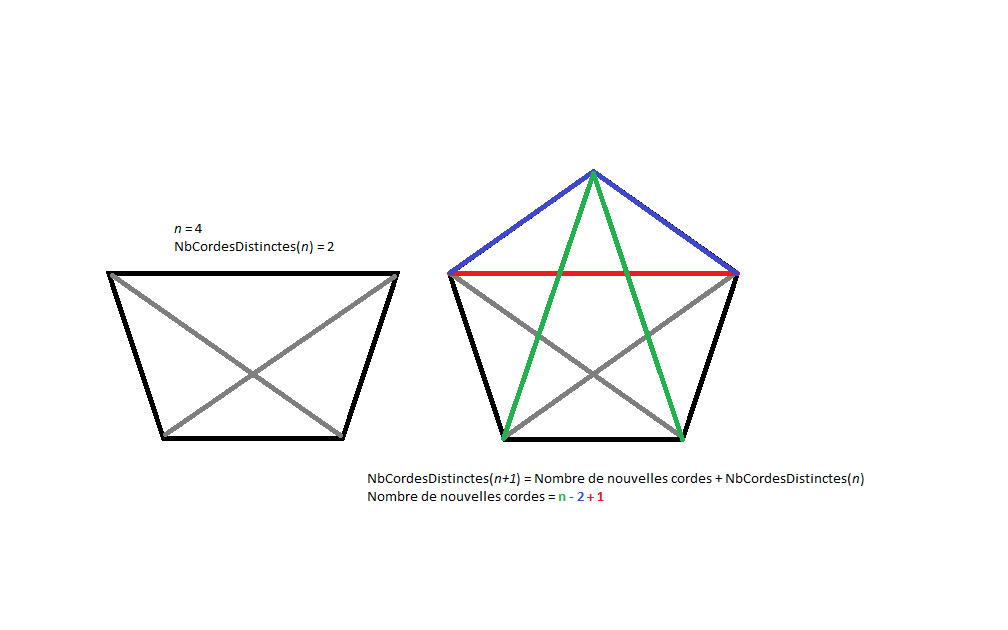
\includegraphics[scale=0.5]{dem1.png}
\caption{Schéma explicatif du nombre de cordes distinctes d'un polygone}
\end{center}
\end{figure}

\[
\begin{array}{r @{=} l}
NbCordesDistinctes(n+1) \ & \ n -  2 + 1 + NbCordesDistinctes(n) \\
			  & \ n - 1 + \frac{n(n-3)}{2} \\
			  & \ \frac{{n^2}-n-2}{2} \\
			  & \ \frac{(n+1)(n-2)}{2} \\
\end{array}
\]
Ce qui achève la récurrence.	
\end{proof}


\subsection{Nombre de cordes pour les triangulation d'un polygone à \emph{n} sommets}

\paragraph{Propriété :}  
Appelons \emph{NbCordesTriang(n)} le nombre de cordes présentent dans une triangulation d'un polygone à \emph{n} sommets.
Toutes les triangulations d'un polygone à \emph{n} sommets comportent le même nombre de cordes \emph{NbCordesTriang(n)}.
De plus nous avons :
\begin{equation} 
NbCordesTriang(n) = n-3
\end{equation}

\begin{proof}
Pour \(n = 4\) nous avons : \(NbCordesTriang(4) = 1 \) la propriété est vérifiée. \\
%TODO : ajouter trop beaux shéma
Admetons la propriété vrais à un rang \emph{n} et démontrons la au rang \emph{n+1}. \\
Considerons un polygone à \emph{n+1} sommets, en traçant une corde entre les sommets \emph{i} et \emph{i+2} on génère un sous polygone de taille \emph{n}.
Le nombre de cordes d'une triangulation d'un polygone de taille \emph{n+1} est donc égale au nombre de cordes du sous polygone de taille \emph{n} au quel on ajoute une corde.
Nous avons :\\
\[
\begin{array}{r @{=} l}
NbCordesTriang(n+1) \ & \  1 corde + NbCordesTriang(n) \\
			  & \ 1 + (n-3) \\
			  & \ (n+1) - 3
\end{array}
\]
Ce qui achève la récurrence.
\end{proof}


\section{Essais successifs}

\subsection{Fonction validecorde()}


Nous utiliserons pour la methode d'essai successif une fonction validecorde nous permettant de savoir si une corde est valide, c'est à dire qu'elle ne coupe pas d'autre corde déjà tracer.

Ce problème se réduit à savoir si une corde en coupe une autre, si la corde donnée ne coupe aucune autre déjà tracé alors elle est valide.

Notons c$(s_a,s_b)$ la corde de sommet A,B avec A$<$B (les sommet étant numéroté et ordonné).

Soit c$(s_a,s_b)$ la corde déjà tracé et c$(s_i,s_j)$ la corde testée.
Si les cordes ne se coupent pas alors il existe 2 cas de figure soit s(i,j) est « au dessus » soit elle est en « dessous » ce qui donne a$<$i;j$<$b (cas au dessous) ou i$<$a j$>$b (au dessus).

Il faut également vérifier que les cordes soient bien distinctes.
 
\subsection{Première Approche}
 

On se place dans une stratégie d'essai successif avec pour choix à l'étape i de prendre une codre valide issue de $s_i$ ou bien de ne rien prendre. 
Cette méthode n'est pas très efficace et donneras souvent plusieur fois la meme trinagularisation. La corde $(s_a,s_b)$ pourra en effet être retennue au passage par l'étape a mais aussi au passage par l'étape b. 
L'exemple le pus simple pour illuster cela est celui du quadrilatère qui ne possède que 2 triangulation, pourtant cette methode en donneras 4.
De plus cette methode ne permet pas de trouver toute les trinagulation contre exemple :
pour n=8, la triangulation $(s_1,s_3),(s_3,s_5),(s_5,s_7),(s_1,s_7),(s_1,s_5)$.
A plus forte raison toute triangulation possédant plus de cordes que de point servant a la trinagulation ne pourras être trouvé via cette méthode.

\subsection{Deuxième Approche} 
\paragraph{Principe Algorithmique :} 
Nous choisierons à l'étape i la corde pour la iéme place de la solution (tableau de solution de taille n-3).
Nous choisirons cette corde parmis les $n(n-3)/2 - k$ cordes restantes avec $k<=i$.
On incrémente k à chaque corde évalué (choisie ou non) de manière a ne jamais retomber deux fois sur la même solution.

\subsection{Mise en oeuvre}

//TODO pseudo code

On suppose connu un tableau de toute les corde tabcorde

\begin{tabbing}
\hspace{0.5cm} \= \hspace{0.5cm}  \= \hspace{0.5cm} \= \hspace{0.5cm} \= \kill


\textit{//initialisation de Exterieur}\\
pour i de 0 à n\\
faire\\
\> Ajouter P[i] à Exterieur\\
finpour\\
\\
\textit{//Boucle principale pour remplir le tableau de solution}\\
pour k de 1 à n-3\\
faire\\
    \> min:= $+\infty$ \\ 
    \> pour i de 0 à n\\
    \> faire\\
        \> \> si P[i] est dans Exterieur\\
        \> \> alors\\
            \> \> \> c:=corde excluant P[i]\\
            \> \> \> si coutcorde(c)<min\\
            \> \> \> alors\\
                \> \> \> \> min:=coutcorde(c)\\
                \> \> \> \> indice:=i\\
                \> \> \> \> solution[k]:=c\\
            \> \> \> finsi\\
        \> \> finsi\\
    \> finpour\\
    \> Retirer P[indice] de Exterieur\\
finpour\\
\end{tabbing}

Cette algorithme possède donc une compléxité temporelle très importante en $O(k^n)$.
Sa compléxité spatiale est en $O(n^2)$.

\subsection{Elagage}

Pour rejeter des appels récursif n'aboutissant pas à une solution il convient de limiter les choix sur les dernières cordes du tableu en effet si a l'étape i$<$n-3 on choisis la corde n*(n-3)/2 alors il ne reste plus aucune candidate pour le reste de la solution, il convient donc de limiter le choix des cordes possible au n*n-3/2 moins les k première et moins les n-3 - i dernières pour les laisser en dernier recours au places restantes. 
De cette manière on évite des appel inutiles.
Une voie d'élagage (non implémenter) est celui de la vérification précoce de l'optimalité.
En triant les cordes par longueur croissante on pourrait voir si une solution partielle à la possiblité d'être une meilleur solution que cellle déja trouvé.
Il suffit de comparer son poid additioner au k-i poids des cordes suivantes, si le resultat est plus grand que le poid de la solution déja sauvgardé alors cette solution partielle ne seras jamais meilleur.

 

\section{Programmation dynamique}

\subsection{Formule de récurrence}



On appelera t la taille du sous-problème débutant au sommet \(s_i\), on défini ainsi le sous problème \(T_{i,t}\).
Pour résoudre le sous problème \(T_{i,t}\) de triangulation d'un polygone par Programmation dynamique nous considererons 3 cas:

\begin{itemize}
 \item Cas 1 : on trace une corde entre les sommets \(s_i\) et \(s_{i+t-2}\), puis l'on résoud le problème \(T_{i,t-1}\).
 \item Cas 2 : on trace une corde entre \(s_{i+1}\) et \(s_{i+t-1}\) puis l'on résoud le problème \(T_{i+1,t-1}\).
 \item Cas 3 : on considère un entier \emph{k} compris entre 2 et \emph{t-k}. On trace deux cordes, une entre \(s_{i}\) et \(s_{i+k}\) et une autre entre \(s_{i+k}\) et \(s_{i+t-1}\).
 Puis l'on résoud les sous problèmes \(T_{i,k+1}\) et \(T_{i+k,t-k}\).
\end{itemize}

On déduit de ces 3 cas la formule de récurrence suivante pour un polygone convexe de taille n: 

\begin{equation} 
T_{i,n} = min 
\begin{pmatrix} 
 longueur(s_i, s_{i+t-2}) + T_{i,n-1} \\
  longueur(s_{i+1}, s_{i+t-1}) + T_{i+1,n-1} \\
  longueur(s_i, s_{i+k}) + longueur(s_{i+k}, s_{i+t-1}) + T_{i,k+1} + T_{i+k,n-k}
\end{pmatrix}               
\end{equation}

Nous calculons ici la longueur d'une corde entre les sommets \(s_i\) et \(s_j\) grace à la fonction \( longueur(s_i, s_j) \). 

Cette formule de récurence va nous permettre de construire grâce à un algorithme dynamique un tableau de solutions.
Lorsque ce tableau sera totalement remplis, on choisira alors la meilleure solution présente dans celui-ci.

\subsection{Algorithme}

On utilise un tableau tabSousPoly qui va contenir des structures qui nous permetrons de trouver la bonne solution (cf Figure 2).

\begin{figure}[h!]
\begin{center}
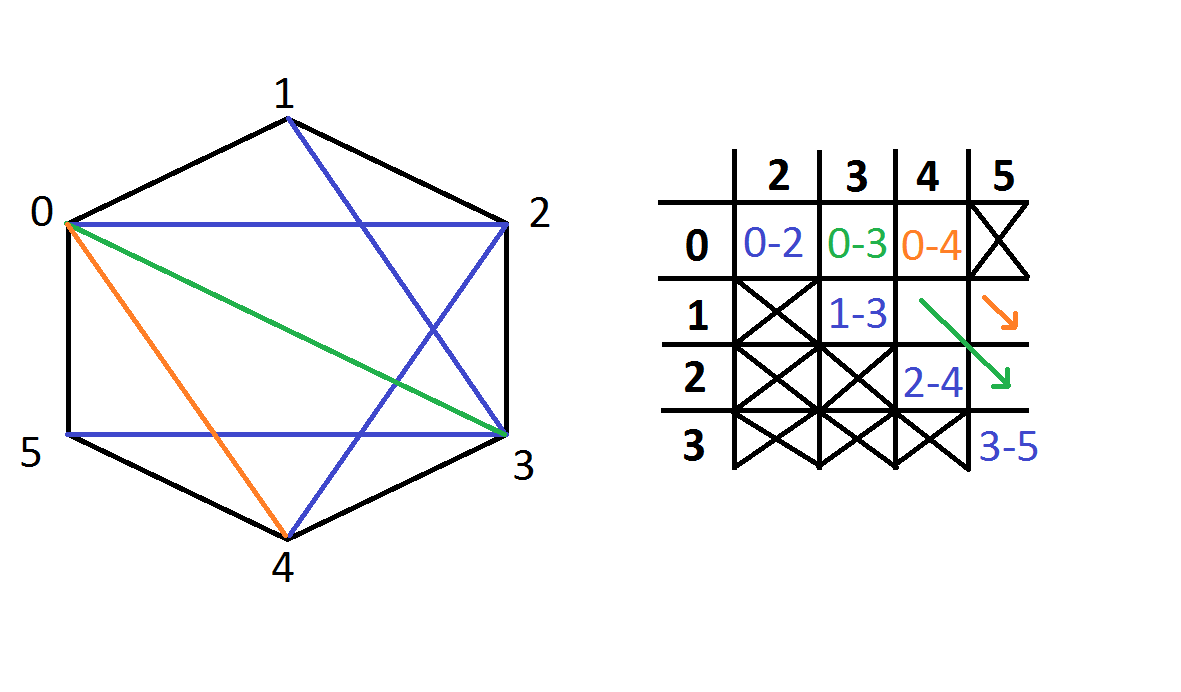
\includegraphics[scale=0.3]{schema1.png}
\caption{Schéma explicatif du tableau de corde d'un polygone pour n=6}
\end{center}
\end{figure}

Cette structure particulière est composée comme suit:
\begin{itemize}
\item ent sommeCorde : correspond à la somme de toutes les cordes ajoutées
 \item ent nbCordes : correspond au nombre total de cordes utilisé pour la triangulation du sous-polygone observé
 \item corde2 *tabCorde : tableau contenant toutes les cordes retenues jusqu'à présent.
\end{itemize}

La structure corde2 quand à elle contient les deux points de la corde et la longueur de celle-ci.

Ainsi dans le tableau tabCorde de la case tabSousPoly[i][j] on enregistre la corde entre les sommets \(s_i\) et \(s_{j+2}\) et le tableau de  corde du sous problème résolue.
  
\begin{tabbing}
\hspace{0.4cm} \= \hspace{0.4cm}  \= \hspace{0.4cm} \= \hspace{0.4cm} \= \hspace{0.4cm} \= \kill

procédure soldynamique(ent n, point poly[], corde2 solution[]); \\
var piou tabSousPoly[n-2][n-2]; \\
var ent i,j,k,x,y, x1, y1; \\
var ent t := 3; \\
var ent NbSommets := 3; //Correspond au nombre de sommets du sous-polygone (au minimum 4) \\
var ent sommeCordeMin; \\
var ent sommeCorde2 ; \\
\\
debut
\textit{//Initialisation de la première diagonale de tabSousPoly}\\
pour i allant de 0 à n-2 faire\\
  \> création de la corde c entre les sommets \(s_i\) et \(s_{i+2}\) \\
  \> tabSousPoly[i][i].sommeCorde := c.lon; \\
  \> \textit{//On ne regarde qu'une seule corde à cette étape} \\
  \> tabSousPoly[i][i].nbCorde := 1; \\
  \> tabSousPoly[i][i].tabCorde[0] := c ; \\
finpour\\
\\
\textit{//Boucle principale pour remplir le tableau tabSousPoly }\\
pour j de 1 à n-3 faire\\
    \> t := t + 1;\\ 
    \> pour i allant de 0 à (n-j-2) faire\\
	\> \> création de la corde c entre les sommets \(s_i\) et \(s_{it-1}\) \\
\> \> \textit{//Cas 1} \\
	\> \> sommeCordeMin = longueur$(s_i, s_{i+t-2})$ + $T_{i,t}$ + c.lon; \\
	\> \> \textit{//On utilise les variables x et y pour garder en mémoire la meilleure case du tableau }\\ 
	\> \> enregistrement des coordonées x y de la case corespondante au cas 1 \\
	\> \> \textit{//Cas 2} \\
	\> \> sommeCorde2 := longueur$(s_{i+1}, s_{i+t-1})$ + $T_{i+1,t}$  c.lon; \\	\> \> si sommeCorde2 $<$ sommeCordeMin alors \\
	  \> \> \> enregistrement des coordonées x y de la case corespondante au cas 2 \\
	\> \> fin si; \\
	\> \> nbCordesArray1 := tabSousPoly[x][y].nbCorde; \\
	\> \> \textit{//Cas 3 : on regarde deux cordes} \\
	\> \> si t $>= 5$ faire \\
	  \> \> \> pour k allant de 2 à NbSommets-3 faire \\
	    \> \> \> \> sommeCorde2 := longueur$(s_i, s_{i+k})$ + longueur$(s_{i+k}, s_{i+t})$ + $T_{i,k+1}$ + $T_{i+k,t-k}$ \\
	    \> \> \> \> si sommeCorde2 $<$ sommeCordeMin alors \\
	      \> \> \> \> \>  enregistrement des coordonées x y de la première case corespondante au cas 3 pour k \\
	      \> \> \> \> \>  enregistrement des coordonées x1 y1 de la deuxième case corespondante au cas 3 pour k \\
	      \> \> \> \> \> enregistrement dans nbCordesArray1 du nombre de corde du premier tableau ajouté \\
	      \> \> \> \> \> enregistrement dans nbCordesArray2 du nombre de corde du deuxième tableau ajouté \\	      
	    \> \> \> \> fin si; \\
	  \> \> \> fait; \\
	\> \> fin si; \\
	\> \> \textit{//Enregistrement de la meilleure solution trouvée }\\
	\> \> tabSousPoly[i][i+j].sommeCorde = sommeCordeMin; \\
	\> \> tabSousPoly[i][i+j].nbCorde = nbCordesArray1 + nbCordesArray2 + 1; \\
	\> \> tabSousPoly[i][i].tabCorde[0] := c ; \\
	\> \> pour k allant de 0 à nbCordesArray1 faire \\
	  \> \> \> tabSousPoly[i][i+j].tabCorde[k+1] := tabSousPoly[x][y].tabCorde[k] ; \\
	\> \> fait; \\
	\> \> si nbCordesArray2 $!=$ 0 faire \\
	  \> \> \> pour k allant de 0 à nbCordesArray2 faire \\
	    \> \> \> \> tabSousPoly[i][i+j].tabCorde[k + nbCordesArray1 + 1] := tabSousPoly[x1][y1].tabCorde[k] ; \\
	  \> \> \> fait;\\
	  \> \> \> nbCordesArray2 := 0;\\
	\> \> fin si; \\
  \> fait; \\
fait; \\
\\
\textit{//Nous venons de finir de remplir la partie du tableau qui nous interresse} \\
\textit{//nous allons maintenant choisir la meilleur solution} \\ 
\textit{//Cas 1} \\
sommeCordeMin = longueur$(s_0, s_{n-2})$ + $T_{0,n-1}$; \\
enregistrement des coordonées x y de la case corespondante au cas 1 \\
\textit{//Cas 2} \\
sommeCordeMin = longueur$(s_1, s_{n-1})$ + $T_{0,n-1}$; \\
si sommeCorde2 $<$ sommeCordeMin alors \\
  enregistrement des coordonées x y de la case corespondante au cas 2 \\
fin si; \\
si n $>=$ 5 faire \\
  \> \textit{//Cas 3 : on regarde deux cordes} \\
  \> pour k allant de 2 à NbSommets-3 faire \\
    \> \> sommeCorde2 := longueur$(s_0, s_{k})$ + longueur$(s_{k}, s_{n-1})$ + $T_{0,k+1}$ + $T_{k,n-k}$ \\
	  \> \> \> si sommeCorde2 $<$ sommeCordeMin alors \\
	     \> \> \> \>  enregistrement des coordonées x y de la première case corespondante au cas 3 pour k \\
	     \> \> \> \>  enregistrement des coordonées x1 y1 de la deuxième case corespondante au cas 3 pour k \\
	     \> \> \> \> enregistrement dans nbCordesArray1 du nombre de corde du premier tableau ajouté \\
	     \> \> \> \> enregistrement dans nbCordesArray2 du nombre de corde du deuxième tableau ajouté \\	      
	  \> \> \> fin si; \\
  \> fait; \\
fin si; \\

\textit{Enregistrement de la solution finale}
pour k allant de 0 à nbCordesArray1 faire \\
  \> solution[k] := tabSousPoly[x][y].tabCorde[k] ; \\
fait; \\
si nbCordesArray2 != 0 faire \\
  \> pour k allant de 0 à nbCordesArray2 faire \\
    \> \> solution[k + nbCordesArray1] := tabSousPoly[x1][y1].tabCorde[k] ; \\
  \> fait;\\
fin si; \\
fin; \\
\end{tabbing}
 
\subsection{Compléxité spatiale et temporelle}

On utilise une structure tabulaire \((n-2)*(n-2)\) que l'on remplie diagonale par diagonale (à l'aide de deux boucle for imbriquées).
Lors du remplissage de ce tableau, on utilise une boucle for pour l'étude de notre 3eme cas explicité précedement. 
Nous avons ainsi une complexitée spatiale en $O(n^3)$.

De plus, ce tableau à deux dimention contient dans chaque case un tableau de dimention t-2 (ou t est la taille du sous-polygone engendré par la corde contenue dans la case).
On obtient ainsi une complexité spatiale en $O(n^3)$.


\subsection{Améliorations possibles}

En considerant le fait que deux sous-problèmes ont toujours un sommet commun, il apparait que les cas 1 et 2 énoncés précédement sont en réalités des cas particuliers du cas 3.
En effet, le cas 1 est équivalent au cas 3 pour $k=t-2$ on crée ainsi la corde $(s_{i}, s_{i+k})$ et la corde $(s_{i+k}, s_{i+t-1})$.
Cependant dans notre recherche de maximum on doit considèrer la longueur de la corde $(s_{i+k}, s_{i+t-1})$ comme null puisqu'il s'agit d'un coté du polygone.
De manière analogue, le cas 2 est équivalent au cas 3 pour $k=1$, on crée les cordes $(s_{i}, s_{i+k})$ et $(s_{i+k}, s_{i+t-1})$.
Et dans notre recherche, la longueur de la corde $(s_{i}, s_{i+k})$ est considérée comme null.

La formule de récurrence de notre algorithme ce limiterait alors au cas 3. Dans l'implémentation de celui-ci nous devrons donner une longueur null aux cotés du sous-polygone. 


\section{Algorithme glouton}


\subsection{Principe algorithmique}

On réduit le problème au seuls choix des cordes extérieures, ce qui revient à choisir la plus courte et ré-iterer sur le sous polygone intérieur ainsi créer.

On s'attend raisonablement à trouver une triangularisation de coût faible, sans pour autant avoir la certitude que celle ci est la plus optimale.

\subsection{Mise en oeuvre}
 

On dispose d'un ensemble « Extérieur » contenant les points constituant le polygone en cour de triangularisation.
On dispose d'un tableau de solution où inscrire les cordes
On dispose d'un tableu des points ordonné (de cardinal n)
On dispose d'un fonction "coutcorde(corde c)" qui renvoie la longueur d'une corde
 
 
 
\begin{tabbing}
\hspace{0.5cm} \= \hspace{0.5cm}  \= \hspace{0.5cm} \= \hspace{0.5cm} \= \kill


\textit{//initialisation de Exterieur}\\
pour i de 0 à n\\
faire\\
\> Ajouter P[i] à Exterieur\\
finpour\\
\\
\textit{//Boucle principale pour remplir le tableau de solution}\\
pour k de 1 à n-3\\
faire\\
    \> min:= $+\infty$ \\ 
    \> pour i de 0 à n\\
    \> faire\\
        \> \> si P[i] est dans Exterieur\\
        \> \> alors\\
            \> \> \> c:=corde excluant P[i]\\
            \> \> \> si coutcorde(c)<min\\
            \> \> \> alors\\
                \> \> \> \> min:=coutcorde(c)\\
                \> \> \> \> indice:=i\\
                \> \> \> \> solution[k]:=c\\
            \> \> \> finsi\\
        \> \> finsi\\
    \> finpour\\
    \> Retirer P[indice] de Exterieur\\
finpour\\
\end{tabbing}
 

Cet algorithme à donc une complexité en $O(n^2)$ (en pratique $O(n^2log(n)$ pour la recherche de la corde excluant P[i], complexité du à notre impléméentation).

Sa complexité spatiale quand à elle est en $O(n)$.

\section{Comparaison}

En comparant l'optimalité de la solution exacte par rapport à celle donnée par l'algorithme glouton nous pouvons observer que même lorsque n augmente sa valeur (ici en pourcentage d'erreur) reste très faible, inférieur à $0,5$ (cf Figure 3).
Ce qui est très acceptable dans la plupart des situations. 
Nous avons réalisé cette étude en moyennant l'erreur sur 1000 comparaison entre triangulation par la methode exacte et celle, approximative de l'algorithme glouton.

\begin{figure}[h!]
\begin{center}
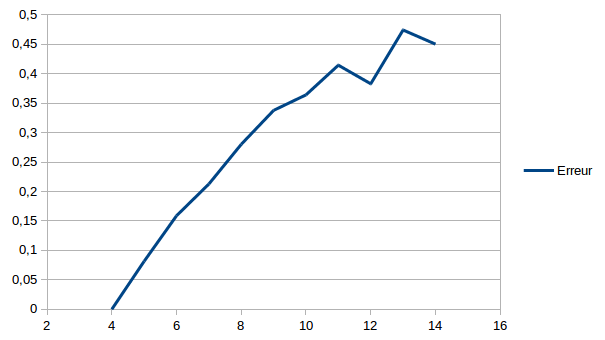
\includegraphics[scale=1]{benchmark2.png}
\caption{Pourcentage d'erreur en donction de n}
\end{center}
\end{figure}

En s'interessant maintenant au temps d'exécution on retrouve bien les différentes classe de compléxité (cf Figure 4).

\begin{figure}[h!]
\begin{center}
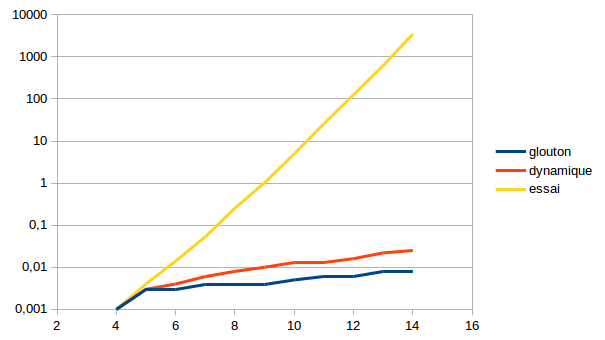
\includegraphics[scale=1]{benchmark.png}
\caption{Temps d'éxécution(ms) en fonction de n (échelle log)}
\end{center}
\end{figure}

Nous voyons bien ici la compléxité exponetielle de l'essai successif.
Nous confirmons aussi la classe de compléxité similaire entre programation dynamique et algorithme glouton avec un nette avantgae pour ce dernier quand n vient a augmenter.

\section{Conclusion}
Les 3 algorithmes proposé dans cette étude (essais successifs, dynamique et glouton), permettent d'obtenir une solution au problème de triangulation de polygones.
Pour les cas de polygones possédants 4 ou 5 côtés, les performances de ces 3 algorithmes sont similaires.
En revanche, on préférera les algorithmes dynamique et glouton à l'essais successif car ce dernier ne donne pas toujours la meilleure solution.
De plus, le temps d'exécution de l'essais successif devient rapidement important lorsque le polygone du problème étudié à plus de 6 coté.

\end{document}

